\documentclass{article}


% if you need to pass options to natbib, use, e.g.:
%     \PassOptionsToPackage{numbers, compress}{natbib}
% before loading neurips_2025


% ready for submission
\usepackage[final]{neurips_2025}


% to compile a preprint version, e.g., for submission to arXiv, add add the
% [preprint] option:
%     \usepackage[preprint]{neurips_2025}


% to compile a camera-ready version, add the [final] option, e.g.:
%     \usepackage[final]{neurips_2025}


% to avoid loading the natbib package, add option nonatbib:
%    \usepackage[nonatbib]{neurips_2025}


\usepackage[utf8]{inputenc} % allow utf-8 input
\usepackage[T1]{fontenc}    % use 8-bit T1 fonts
\usepackage{hyperref}       % hyperlinks
\usepackage{url}            % simple URL typesetting
\usepackage{booktabs}       % professional-quality tables
\usepackage{amsfonts}       % blackboard math symbols
\usepackage{nicefrac}       % compact symbols for 1/2, etc.
\usepackage{microtype}      % microtypography
\usepackage{xcolor}         % colors
\usepackage{import}
\usepackage{graphicx}

\usepackage{amsmath}
\usepackage{subcaption}
\usepackage{multirow}
\usepackage{fancyhdr}
\usepackage{color}
\usepackage{algorithm}
% \usepackage{algorithmic}
% \usepackage{algorithmicx}
% \usepackage{algorithm}
\usepackage{algpseudocode}
\usepackage{adjustbox}
\usepackage{wrapfig}
\usepackage{fontawesome}

\newcommand{\ZJ}[1]{\textcolor{blue}{[ZJ: #1]}}{\ignorespaces}
\newcommand {\aurick}[1]{{\color{cyan}\sf{[AQ: #1]}}}
\newcommand{\go}[1]{{\textcolor{orange}{GO: #1}}}

\title{SuffixDecoding: Extreme Speculative Decoding for Emerging AI Applications}
% \title{\adjustbox{valign=c}{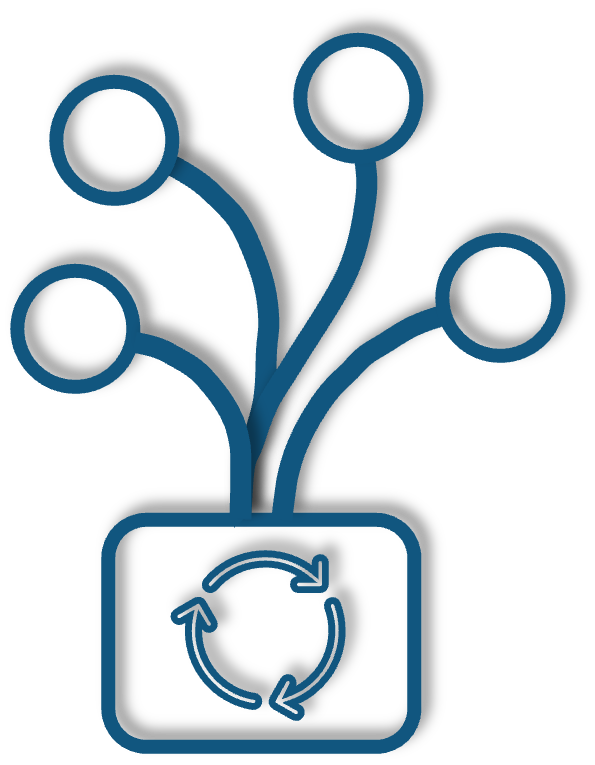
\includegraphics[height=2em]{latex/figures/suffix-logo-min.png}} SuffixDecoding: Extreme Speculative Decoding\\for Emerging AI Applications}



\author{
  \textbf{Gabriele Oliaro}$^{\mathsection,\dag}$
  \quad
  \textbf{Zhihao Jia}$^{\dag}$
  \quad
  \textbf{Daniel Campos}$^{\mathsection}$
  \quad
  \textbf{Aurick Qiao}$^{\mathsection}$
  \\
  ${}^\mathsection$Snowflake AI Research \quad 
  ${}^\dag$Carnegie Mellon University\\
    \texttt{\{goliaro,zhihaoj2\}@cs.cmu.edu}, \\ 
    \texttt{\{daniel.campos,aurick.qiao\}@snowflake.com}\\\\
    \faHome \textbf{ Project Page: }\url{https://suffix-decoding.github.io}\\
    \faGithub \textbf{ Code: }\url{https://github.com/snowflakedb/ArcticInference}
}


\begin{document}


\maketitle


\begin{abstract}
Speculative decoding is widely adopted to reduce latency in large language model (LLM) inference by leveraging smaller draft models capable of handling diverse user tasks. However, emerging AI applications, such as LLM-based agents, present unique workload characteristics: instead of diverse independent requests, agentic frameworks typically submit repetitive inference requests, such as multi-agent pipelines performing similar subtasks or self-refinement loops iteratively enhancing outputs. These workloads result in long and highly predictable sequences, which current speculative decoding methods do not effectively exploit. To address this gap, we introduce \emph{SuffixDecoding}, a novel method that utilizes efficient suffix trees to cache long token sequences from prompts and previous outputs. By adaptively speculating more tokens when acceptance likelihood is high and fewer when it is low, SuffixDecoding effectively exploits opportunities for longer speculations while conserving computation when those opportunities are limited. Evaluations on agentic benchmarks, including SWE-Bench and Text-to-SQL, demonstrate that SuffixDecoding achieves speedups of up to 5.3$\times$, outperforming state-of-the-art methods---2.8$\times$ faster than model-based approaches like EAGLE-2/3 and 1.9$\times$ faster than model-free approaches such as Token Recycling. SuffixDecoding is open-sourced at \url{https://github.com/snowflakedb/ArcticInference}.
\end{abstract}

\subimport{latex/}{s1-introduction.tex}
\subimport{latex/}{s2-background.tex}
\subimport{latex/}{s3-suffix-decoding.tex}
\subimport{latex/}{s4-evaluation.tex}
\subimport{latex/}{s6-conclusion.tex}


{
\small
\bibliography{latex/suffix_decoding}
\bibliographystyle{plainnat}
}

%%%%%%%%%%%%%%%%%%%%%%%%%%%%%%%%%%%%%%%%%%%%%%%%%%%%%%%%%%%%

\newpage
\appendix
\subimport{latex/}{s99-appendix}

%%%%%%%%%%%%%%%%%%%%%%%%%%%%%%%%%%%%%%%%%%%%%%%%%%%%%%%%%%%%

\newpage

\subimport{latex/}{s98-checklist}

%%%%%%%%%%%%%%%%%%%%%%%%%%%%%%%%%%%%%%%%%%%%%%%%%%%%%%%%%%%%

\end{document}